\documentclass{article}
\usepackage[utf8]{inputenc}
\usepackage[a4paper, margin=2cm]{geometry}
\usepackage{indentfirst}
\usepackage{graphicx}
\usepackage{hyperref}
\usepackage{csquotes}
\usepackage{subfig}
\usepackage{color}

\title{Uliège eShop \\e-commerce and e-business project}
\author{Beguin Mathias - Lejoly Loic \\ Github access: \url{https://github.com/MTHSBGN/e-commerce}}
\date{November 2018}

\begin{document}

\maketitle
\newpage

\section{Introduction}
For this project, we decided to work on the proposition given in the statement (Uliège eShop). As asked in the statement the goal is to provide a website where objects related to the University can be sold. To achieve that, we decided to use a relational database to store products and data related to customers. Concerning the back-end's website, PHP and JavaScript are used. Javascript is essentially used as a REST API for GET requests. The benefit of that is this API can be used by third part apps without giving access to them to change the database. Concerning the front-end part as usual HTML,CSS and JS are used.

\section{Database architecture}
To model the database of the Uliège eShop website a relational database architecture was chosen because the product catalogue is not large and because it can be hard to have a good NO-SQL design. On the web you can find some debate that discuss the fact to use relational DB or no-SQL DB. The advantage of the no-SQL DB is that it is easier to manage your product catalogue (product variations) but the drawback of no-SQL DB is the reliability (can be solved with DB clustering e.g: foundationdb, couchDB,...). Concerning the reliability relational DB architectures are, for the majority, ACID compliant. These two types of architectures are not mutual exclusive. Most of the time, e-commerce websites use of combination of SQL and No-SQL DBs (a paper discussing that topic \url{https://aisel.aisnet.org/cgi/viewcontent.cgi?article=1026&context=sais2013}).

\subsection{entity-relationship model}
\autoref{ecommerce_er} depicts the entity-relationship model based on the minimal requirements given in the statements. We decided to split the product table proposed in the statement into multiple tables to avoid data replications and to provide a scalable approach. Indeed, in the product table proposed, all data linked to a product is packaged into this table. The result of that is it is difficult to manage products with different properties (e.g colors, size,...) without replications. That is why we decided to split this table into several tables that are \textit{Sku (stock keeping units) Variant (gives the properties of a product), Description (Give the product description), and Category (specify the product category)}. \\

Concerning the transaction part we decided to split that part into two related steps. The first step establishes a relation between the sku ID and the order ID (defined in the second step) and specifies the quantity needed. This step is achieved with the table Order\_details. The second step consist in summarizes the the order of the client by referencing the ID of the order, the delivery address, the total price of the order, and  the user ID.

\subsection{Relational model}
\begin{enumerate}
\item Customer(client\_id, mail, username,password, delivery\_address, first\_name, last\_name)

\item Client\_order(order\_id, \#client\_id, date, total\_price, ship\_address)

\item Order\_details(\#order\_id, \#sku\_id, quantity)

\item Sku(sku\_id, \#produt\_id, price, available, sold)

\item Variants(variant\_id, attribute, value)

\item Description(description\_id,  french,  english)

\item Category(category\_id, \#description\_id, name)
\end{enumerate}

\begin{figure}[h!]
    \centering
    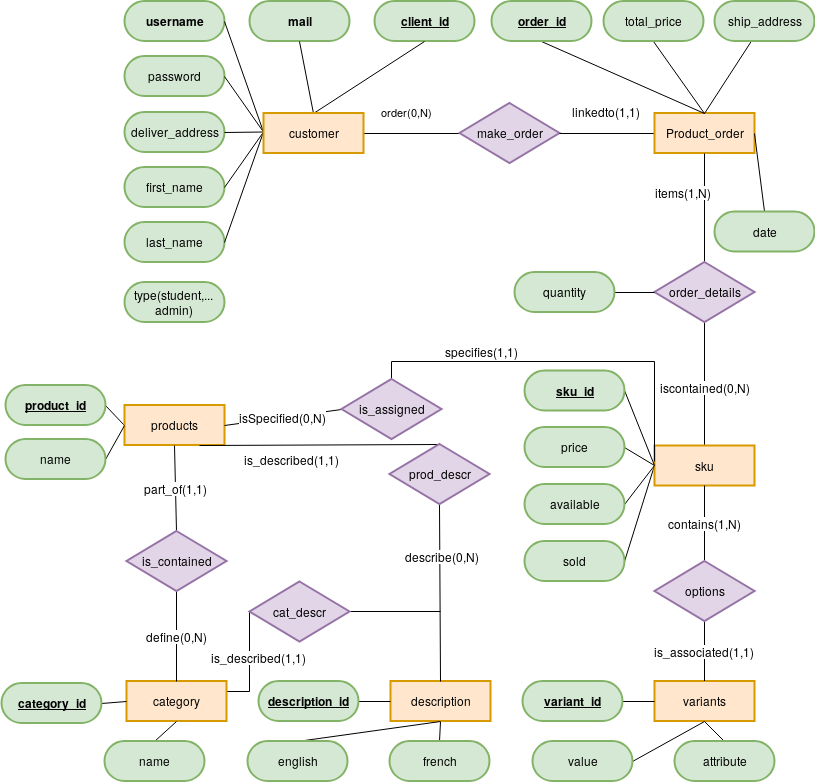
\includegraphics[scale=0.4]{./images/ecommerce_ER.png}
    \caption{eShop entity-relationship model}
    \label{ecommerce_er}
\end{figure}

\subsection{model to SQL tables}
The translation of the model depicted on \autoref{ecommerce_er} can be translated into SQL tables as \autoref{ecommerce_sql} shows. If you want a more interactive view of these tables, you can load the sql file in \textit{phpmyadmin} for instance.

\begin{figure}[h!]
    \centering
    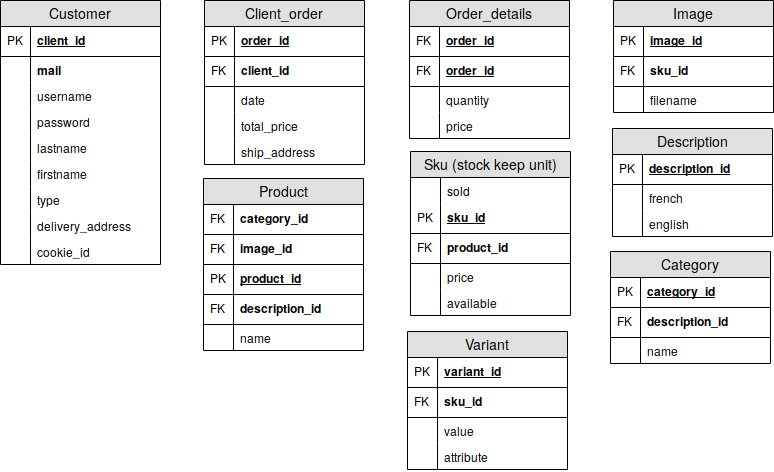
\includegraphics[scale=0.4]{./images/ecommerce_SQL.png}
    \caption{eShop entity-relationship model}
    \label{ecommerce_sql}
\end{figure}

\section{Website}
The website is divided into section. The first section is dedicated to the admin of the website itself an can only be accessed by users with the right privileges. The second second is dedicated to customer where they can buy products. For the development of the website we applied minimal protections like SQL injection and direct PHP scripts access protections.

\subsection{Admin panel}
The admin panel is a dashboard provided to the administrator of the website. The users that can use this panel have special privileges. To detect this kind of users the field type of customer table is set to zero. As results, a admin user needs to follow the regular registration phase to create an account and then the super user that has a direct access to the database can change the type field to promote a user as admin user. Admin users have an extra button to allow them to access to the admin panel.\\

The dashboard is simple at left a menu can help the user to navigate through the different webpages. As you can see on the \autoref{fig:admin} the panel only contains 3 pages (home,product,category). The homepage summarizes different parameters, you can also export some data. The product and Category pages give the possibility to add new elements to the database easily. \\

Even if you are on the dashboard you can go back to the e-commerce pages just by clicking on the website button.

\begin{figure}[h!]
    \centering
    \subfloat[admin homepage]{{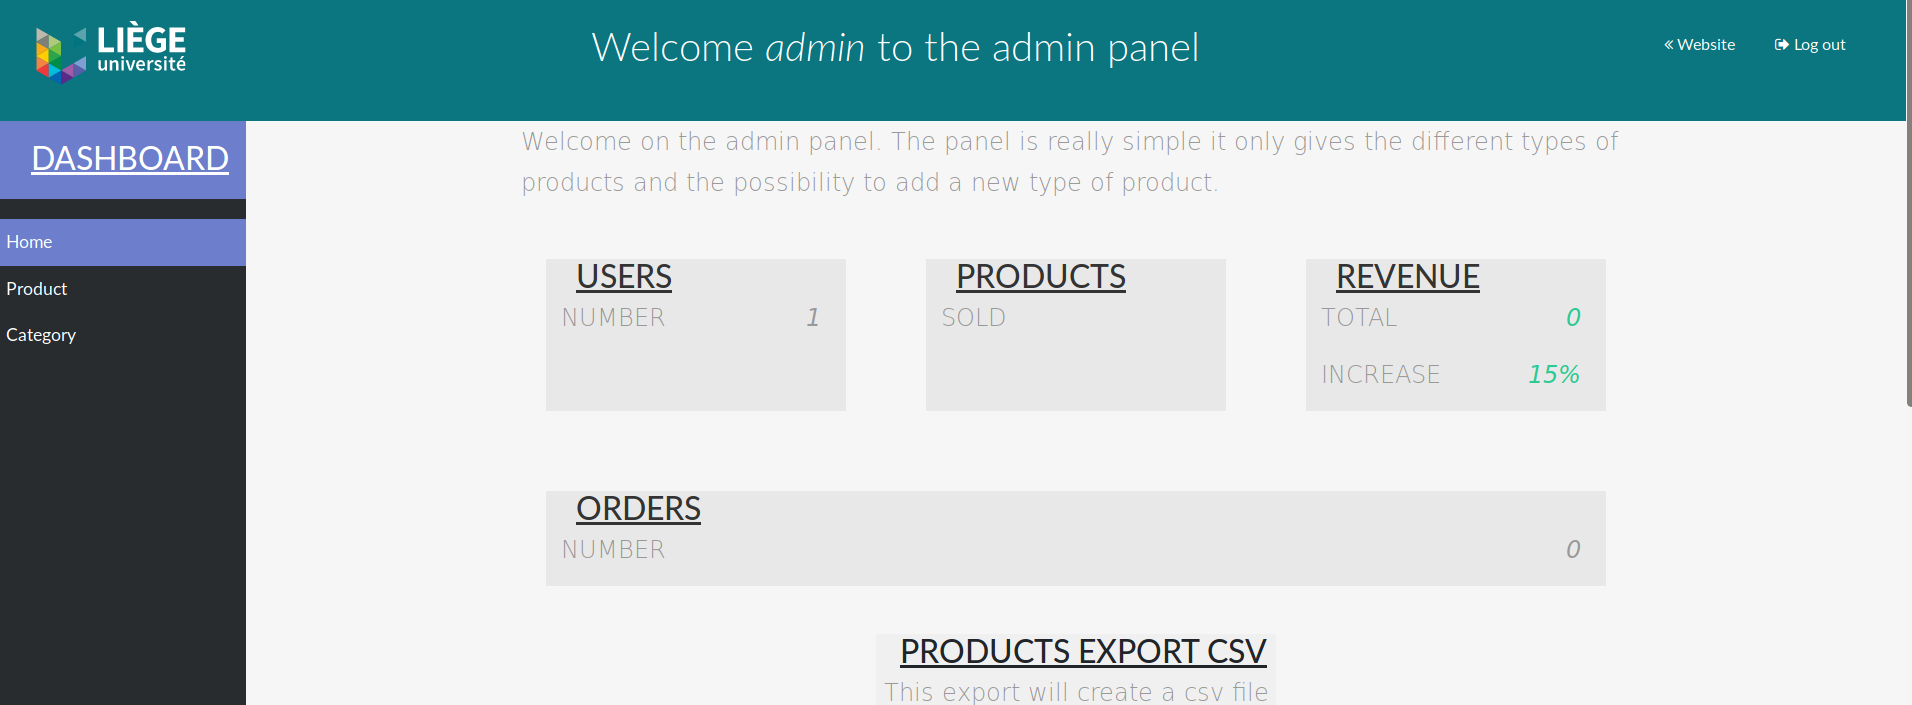
\includegraphics[scale=0.2]{./images/index_admin.png}}}%
    \qquad
    \subfloat[product manager]{{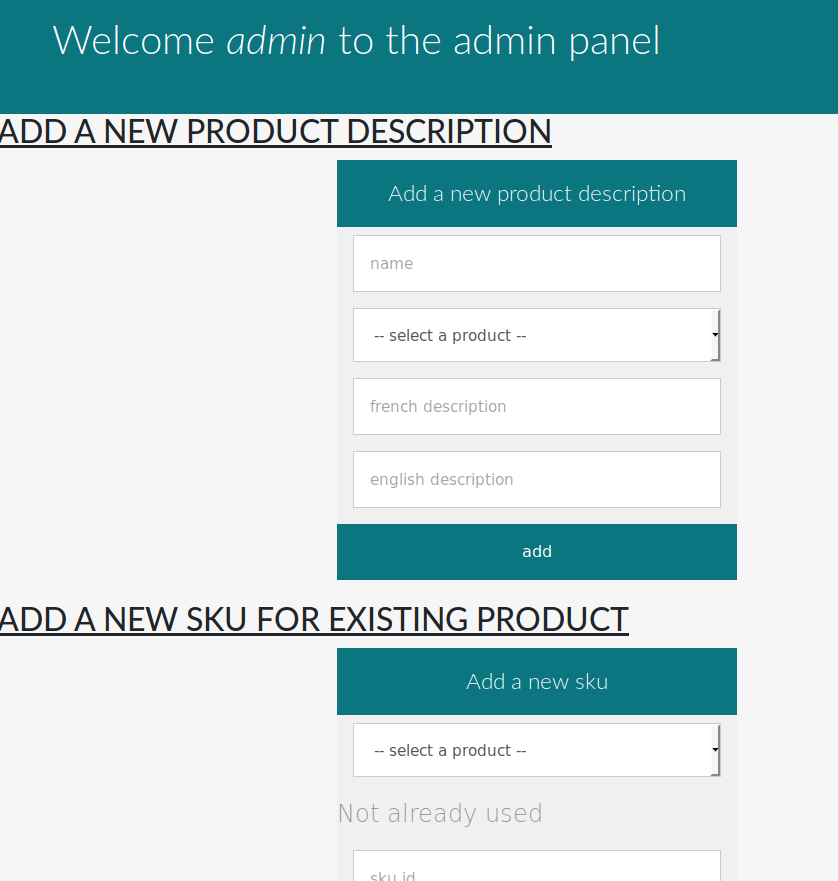
\includegraphics[scale=0.3]{./images/product_admin.png}}}%
    \caption{admin pages}%
    \label{fig:admin}%
\end{figure}

\subsection{Customer View}
%Explain a bit the catalog page

\subsubsection{Registration}
To purchase products, a customer needs to create an account on the website to do so, he needs to click on the button dedicated to that purpose or simply follow \textit{http://websitedomain.com/register.php}. On that page the user must fill fields with correct informations and then validate his account. If everything is correct, he is redirected to the login page.
 
\subsubsection{Log in}
After the creation of an account a user can connect to the website by using his account informations. To achieve that he simply click on the button made for that purpose or going to \textit{http://websitedomain.com/login.php}. If the information given are correct he will be redirected on the home page.
 

\begin{figure}[h!]
    \centering
    \subfloat[register page]{{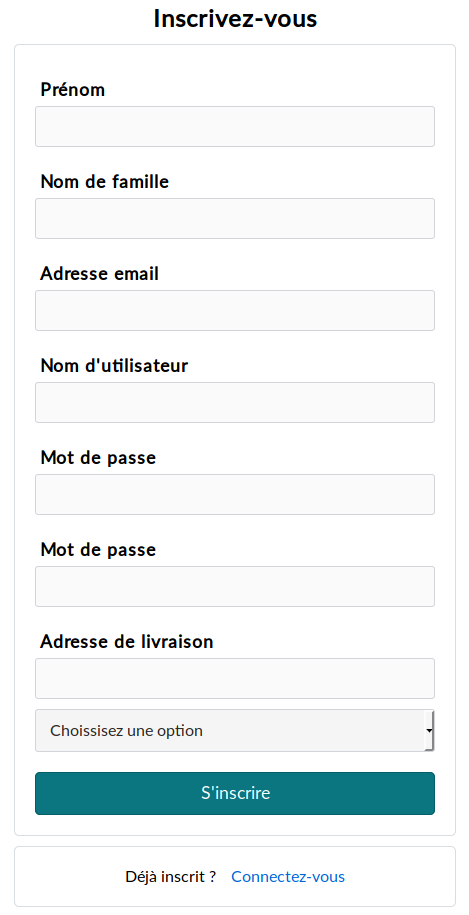
\includegraphics[scale=0.3]{./images/sign_up.png}}}%
    \qquad
    \subfloat[login page]{{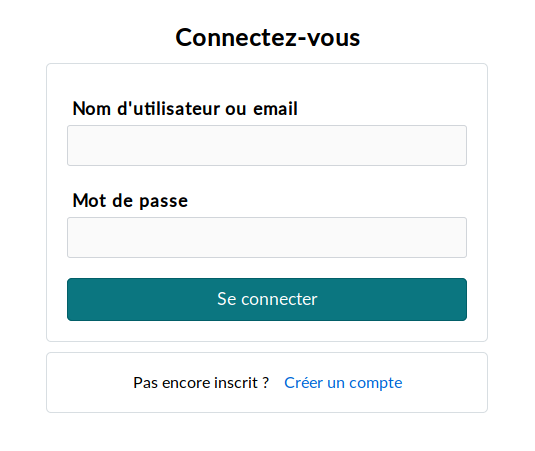
\includegraphics[scale=0.3]{./images/sign_in.png}}}%
    \caption{connection pages}%
    \label{fig:mineral}%
\end{figure}

The login page is the same for the admin, since the admin has more privileges when he is logged, he can access more pages such has the admin panel.

\subsection{Basket}
% Put a description

\subsubsection{Payment}
Since none payment procedure like PayPal etc. is set, a simple payment page is used to update the database. Even if it is a simple page, a transactional commit phase is established to be sure that all tables are updated correctly.

\subsection{Security aspects}
Concerning the security of the website, some common guidelines are applied such as SQL injections, forbid direct access to .php pages only done in some php scripts but must be done on server part also, especially for DB script accesses. As discussed above transactional commit is done for the payment page.

\end{document}

